% MIT License

% Copyright (c) 2022-23 Melonbob (Robert F. Burgie)

% Permission is hereby granted, free of charge, to any person obtaining a copy
% of this software and associated documentation files (the "Software"), to deal
% in the Software without restriction, including without limitation the rights
% to use, copy, modify, merge, publish, distribute, sublicense, and/or sell
% copies of the Software, and to permit persons to whom the Software is
% furnished to do so, subject to the following conditions:

% The above copyright notice and this permission notice shall be included in all
% copies or substantial portions of the Software.

% THE SOFTWARE IS PROVIDED "AS IS", WITHOUT WARRANTY OF ANY KIND, EXPRESS OR
% IMPLIED, INCLUDING BUT NOT LIMITED TO THE WARRANTIES OF MERCHANTABILITY,
% FITNESS FOR A PARTICULAR PURPOSE AND NONINFRINGEMENT. IN NO EVENT SHALL THE
% AUTHORS OR COPYRIGHT HOLDERS BE LIABLE FOR ANY CLAIM, DAMAGES OR OTHER
% LIABILITY, WHETHER IN AN ACTION OF CONTRACT, TORT OR OTHERWISE, ARISING FROM,
% OUT OF OR IN CONNECTION WITH THE SOFTWARE OR THE USE OR OTHER DEALINGS IN THE
% SOFTWARE.
\documentclass{article}
\usepackage[letterpaper,portrait]{geometry}
\pagenumbering{gobble}
\usepackage{pgfplots,textcomp}
\pgfplotsset{width=12cm,compat=1.15}
\begin{document}
% 3-step: beta rest mash-in, TmodRIMS; 2INF-modRIMS in alpha; 3INF mash-out
% b-TR-I-TR-I
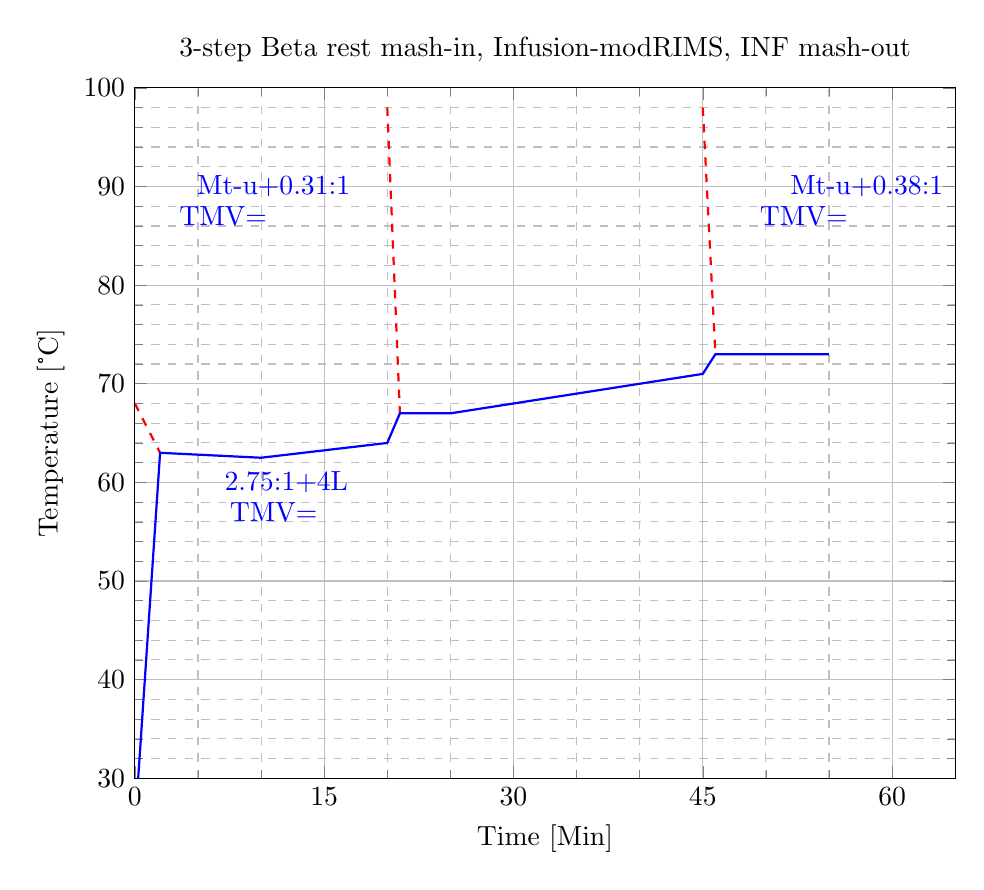
\begin{tikzpicture}
\begin{axis}[
  title={3-step Beta rest mash-in, Infusion-modRIMS, INF mash-out},
  xlabel={Time [Min]},
  ylabel={Temperature [\textdegree{C}]},
  xmin=0, xmax=65,
  ymin=30, ymax=100,
  xtick={0,15,30,45,60,75,90,105,120},
  ytick={30,40,50,60,70,80,90,100},
  % legend pos=north west,
  ymajorgrids=true,
  xmajorgrids=true,
  grid style=thin,
  %grid=major,
  minor grid style=dashed,
  yminorgrids=true,
  xminorgrids=true,
  yminorticks=true,
  xminorticks=true,
  minor y tick num=4,
  minor x tick num=2
]
\addplot [color=red, style=dashed,thick]
  coordinates {
   (0,68)% strike temp
   (2,63)% mash-in 2.75:1 (44+4L on PR1 w/ 16kg) TMV=48+0.67*16=59L
  };
\node [color=blue] at (axis cs:12,60) {2.75:1+4L};
\node [color=blue] at (axis cs:11,57) {TMV=};
\addplot [color=red, style=dashed,thick]
  coordinates {
   (20,98)(21,67)% 2INF 0.31:1 (5L on PR1 w/ 16kg) TMV=64L
  };
\node [color=blue] at (axis cs:11,90) {Mt-u+0.31:1};
\node [color=blue] at (axis cs:7,87) {TMV=   };
\addplot [color=red, style=dashed,thick]
  coordinates {
    (45,98)(46,73)% 3INF 0.38:1 (7L on PR1 w/ 16kg) TMV=71L
  };
\node [color=blue] at (axis cs:58,90) {Mt-u+0.38:1};
\node [color=blue] at (axis cs:53,87) {TMV=   };		
\iffalse% block comment		               not used from here
\addplot [color=green, style=thick]
  coordinates {
   (70,64.5)(95,99)(105,99)
  };
\addplot [color=green, style=dashed,thick]
  coordinates {
    (105,99)(107,77)
  };
\fi%    					                     to here
\addplot [color=blue, style=thick]
  coordinates {
    (0,25)% initial grist temp
    (2,63)% mash-in
    (10,62.5)% beta rest 10'
    (20,64)% TmodRIMS 1C/5min, cooling loss w/o -4C/hr=-1C/15min
    (21,67)% 2INF  0.31:1 5L on PR1
    (25,67)% 5' alpha rest, no cooling loss with RIMS
    (45,71)% TmodRIMS 1C/5min
    (46,73)% 3INF 0.38:1 7L on PR1, mash-out
    (50,73)% 5' Lauter/ mash bed settle/ no RIMS
    (55,73)% 5' Vorlauf/ no hose
  };
%\legend{}
 
\end{axis}
\end{tikzpicture}
\end{document}